\section{A ground truth for clustering} \label{sec:Comparison_Clustering}

Since the use of $k$-mer frequencies proved to be valid for \gls{IAV} clustering, further investigation on the source of the persisting errors \autoref{fig:PCA_Cluster_Knee_4} \textbf{\textsf{B}} and \textbf{\textsf{D}} was performed. For investigation standard \texttt{HDBSCAN} clustering was used without hybrid setting and $\varepsilon$ exploration on the same small subset of H13 and H16 sequences used in the previous section. Standard \texttt{HDBCSCAN} was used for simplification and minimization of error sources. Also, the subset used with 662 sequences was smaller than e.~g.~, the one for full segment 4 clustering with 56617 sequences, making the use of hybrid \texttt{HDBSCAN} unnecessary. 

\vspace{1em}

Two different clusterings on this small subset, without the necessity of any dimension reduction were performed and compared to find a ground truth. Subsequently the results were compared to a clustering on the same subset with a simple version of the PK method and, therefore, involvement of dimension reduction. The first input was the non-reduced set of $k$-mer frequency vectors used in \autoref{sec:K_mer_Representation} as precalculated cosine distance matrix (\autoref{fig:Precalc_Pipeline} workflow \textsf{\textbf{8}}). \texttt{HDBSCAN} can use precalculated distances as input instead of vectors. Therefore, no distance calculation is performed by \texttt{HDBSCAN}. Precalculated distances on $n$ vectors create matrices of size $n \times n$, therefore, precalculation is very RAM intensive and not usable on a high number of sequences. Still, since this approach involved no dimension reduction and less calculation by the clustering tool, thereby less error sources, the resulting clustering could be used as ground truth. The result of the clustering was visualized as clustering tree (\autoref{fig:Simple_Clustertree_Cosine}). 

\begin{figure}[!hbt]
    \centering
    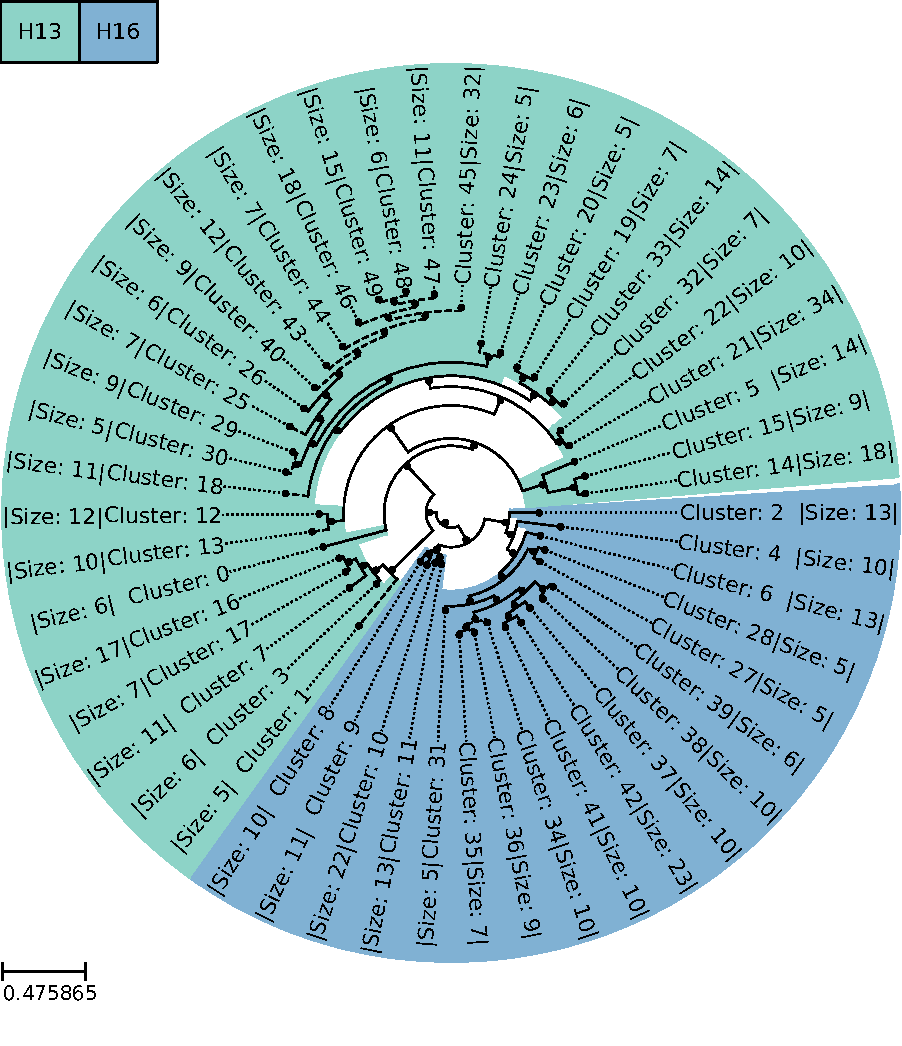
\includegraphics[width=\textwidth]{PCA/Clustertree_Segment_4_H_Cosine.pdf}
    \caption[Simple clustering tree of H13/H16 with cosine distance]{\textbf{Simple clustering tree of H13/H16 with cosine distance.} Clustering tree, based on the clustering by standard \texttt{HDBSCAN} without $\varepsilon$ exploration and hybrid clustering. The matrix used as input contained precalculated cosine distances. The distances were calculated from the $k$-mer frequency vectors related to the sequences, present in the H13 and H16 clusters in \autoref{fig:PCA_Clusteree_Knee_4} without reduction with \texttt{PCA} or \texttt{UMAP}. Therefore, \texttt{HDBSCAN} was used with precalculation input instead of a distance metric.}
    \label{fig:Simple_Clustertree_Cosine}
\end{figure}

\begin{figure}[!hbt]
    \centering
    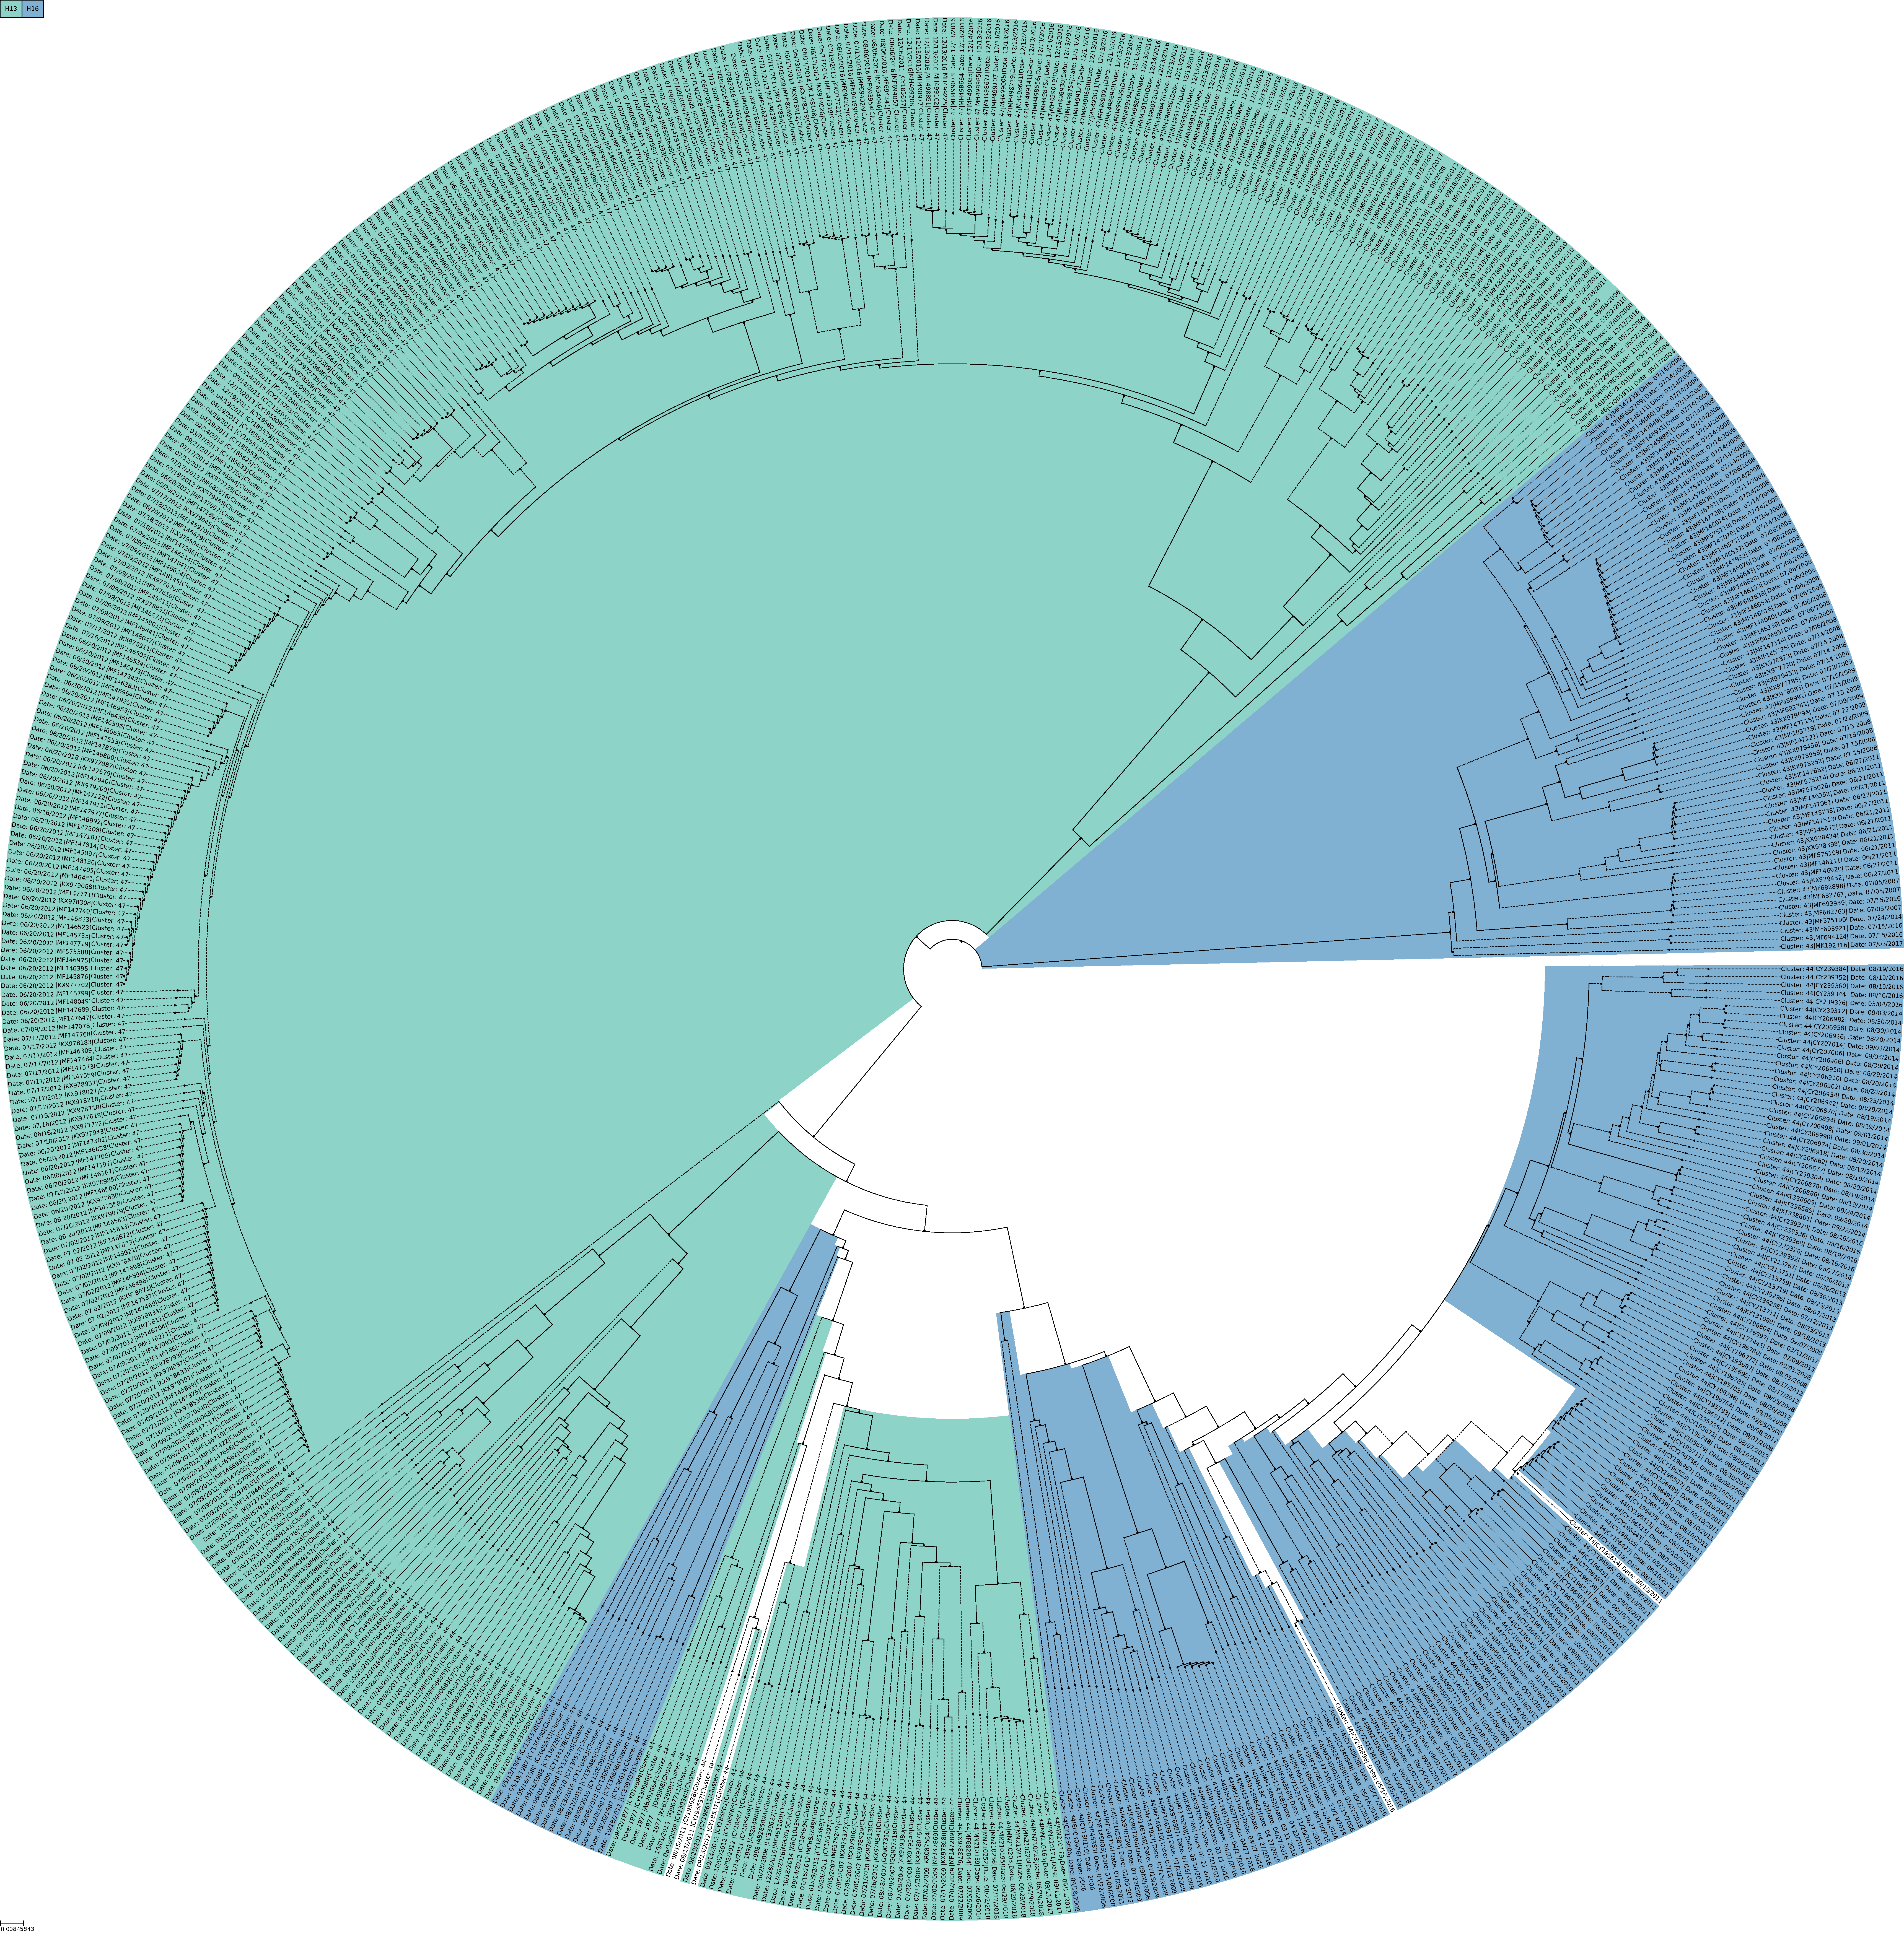
\includegraphics[width=\textwidth]{PCA/Clustertree_Segment_4_H_Focus.pdf}
    \caption[Simple clustering tree of H13/H16 with evolutionary distance]{\textbf{Simple clustering tree of H13/H16 with evolutionary distance.} Clustering tree, based on the clustering by standard \texttt{HDBSCAN} without $\varepsilon$ exploration and hybrid clustering. The matrix used as input contained precalculated \gls{MSA} based evolutionary distances. The sequences, present in the H13 and H16 clusters in \autoref{fig:PCA_Clusteree_Knee_4} were used for the \gls{MSA}. Therefore, \texttt{HDBSCAN} was used with precalculation input instead of a distance metric.}
    \label{fig:Simple_Clustertree_MSA}
\end{figure}

\begin{figure}[!hbt]
    \centering
    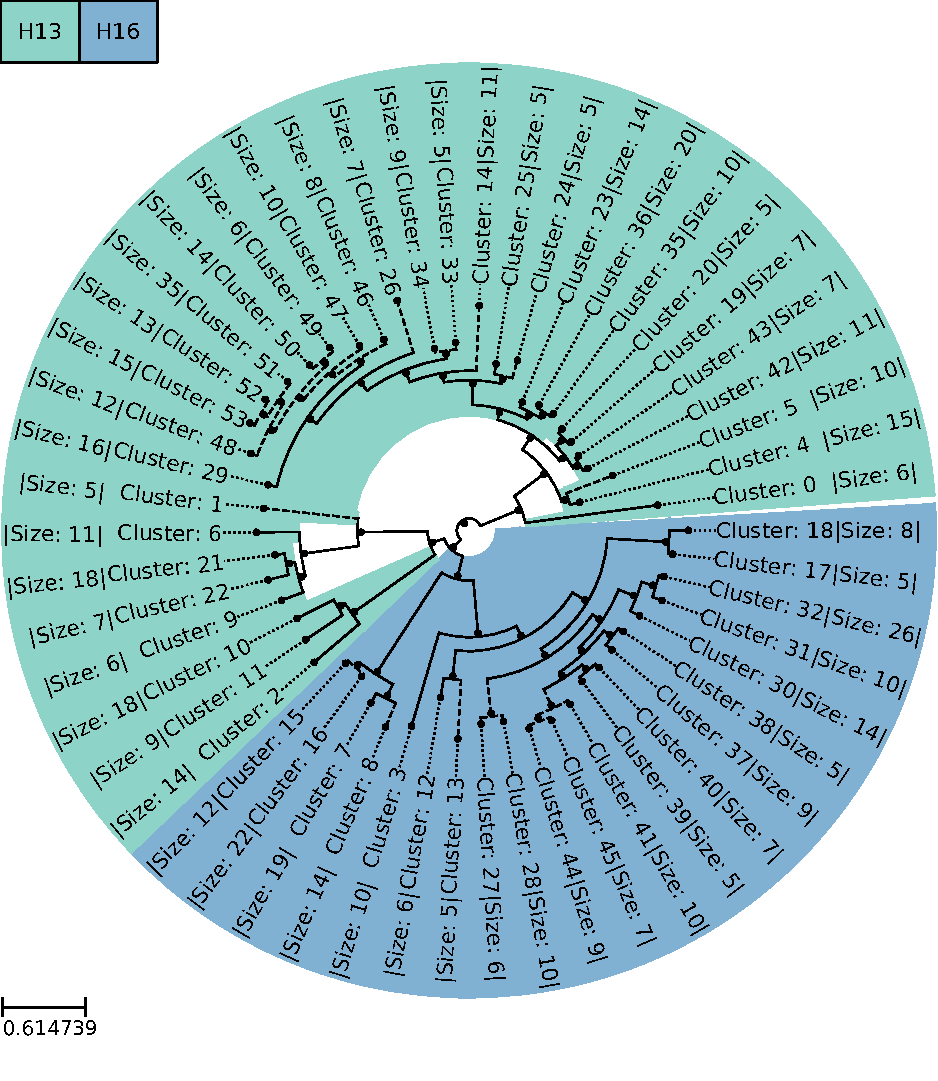
\includegraphics[width=\textwidth]{PCA/Clustertree_Segment_4_H_Simple.pdf}
    \caption[Simple clustering tree of H13/H16 with PCA]{\textbf{Simple clustering tree of H13/H16 with PCA.} Clustering tree, based on the clustering by standard \texttt{HDBSCAN} without $\varepsilon$ exploration and hybrid clustering. The used vectors were related to the sequences, present in the H13 and H16 clusters in \autoref{fig:PCA_Clusteree_Knee_4} and reduced by \texttt{PCA} to 30 dimensions.}
    \label{fig:Simple_Clustertree_PCA}
\end{figure}

\vspace{1em}

In a similar manner to the precalculated \gls{UPGMA} tree in \autoref{fig:Precalculated_Cosine}, the subtypes in \autoref{fig:Simple_Clustertree_Cosine} are completely separated and split on both sides in two subgroups. This pointed to the fact, that the \texttt{HDBSCAN} clustering of the precalculated cosine distances of the $k$-mer frequencies are as usable as the $k$-mer frequencies itself to draw a clear line to separate the subtypes. This finding is in line with the second clustering tree based on similar clustering on the same sequences with evolutionary distances of a \gls{MSA} instead (\autoref{fig:Alignment_Pipeline} workflow \textsf{\textbf{6}}). There, the same separation is even more obvious, as the subtypes subtrees are farther away from the separation at the trees root in \autoref{fig:Simple_Clustertree_MSA}. On the side of the H13 sequences, a subdivision is also clearly noticeable. Subgroups in the H16 sequences are, on the other hand, not that clear separated. The different distances between the subtypes and the subgroups in \autoref{fig:Simple_Clustertree_Cosine} and \autoref{fig:Simple_Clustertree_MSA} were most likely caused by evolutionary aspects integrated in the calculation of distances by the \gls{MSA}. By the $k$-mer frequencies, the pure constellation of nucleotides was used, evolutionary aspects were neglected. However, clustering with the precalculated approach as well as with the \glspl{MSA} evolutionary distances used the full information available from the sequences themselves. No reduction with \texttt{PCA} or \texttt{UMAP} was performed and both clustering trees indicate full subtype separation. Therefore these clustering trees (\autoref{fig:Simple_Clustertree_Cosine} and \autoref{fig:Simple_Clustertree_MSA}) were the only ground truth for H13/H16 clustering with \texttt{HDBSCAN} available. As already mentioned precalculated clustering with \texttt{HDBSCAN}, is highly computationally expensive, as the matrices of size $n \times n$ have to be calculated and saved to be used in \texttt{HDBSCAN}. The calculation is, therefore, not possible without the availability of major RAM space. When using \texttt{HDBSCAN} with the $k$-mer vectors posterior to reduction with \texttt{PCA} to 30 dimensions, only a matrix of size $n\times 30$ has to be saved without the necessity of any distance precalculation. This is a \textbf{major} reduction of computational power necessary. 

\vspace{1em}

A third clustering was performed using \texttt{PCA} reduced vectors of the same H13/H16 sequences (\autoref{fig:Simple_Pipeline}). To validate the accuracy of the dimension reduction by \texttt{PCA}, used in this project, the clustering tree in \autoref{fig:Simple_Clustertree_PCA} should have represented the ground truth of the previous trees as best as possible. As described in \autoref{sec:Clustering}, the method using \texttt{PCA} and the Kneedle Algorithm was declared as best method for \gls{IAV} clustering (PK). In this comparison by standard \texttt{HDBSCAN} clustering without $\varepsilon$ exploration, the sole reduction with \texttt{PCA}, representing simplified PK method was, therefore, used (\autoref{fig:Simple_Clustertree_PCA}). Unfortunately, some major differences between the clustering trees using \texttt{PCA} and the two trees using precalculated cosine distance and \gls{MSA} evolutionary distance stood out. In \autoref{fig:Simple_Clustertree_PCA}, the whole tree of H16 is first joined to a subtree of H13, before joining to the other H13 subtree. Therefore, no clear separation is present. The same clustering behavior, without a clear separation was observed in the complete clustering tree in the previous section (\autoref{fig:PCA_Clusteree_Knee_4} \textbf{\textsf{B}}). The euclidean distance calculation included in the mutual reachability distance of \texttt{HDBSCAN} is related to the cosine distance as proven in \autoref{chap:Materials_and_Methods}. Furthermore, the Kneedle Algorithm was not used as no $\varepsilon$ exploration was performed. Thus, excluding the distance calculation and the Kneedle Algorithm from the error sources. Thereby, the \texttt{PCA} dimension reduction step seemed to be the origin of the clustering error in \autoref{fig:PCA_Cluster_Knee_4} \textbf{\textsf{B}} and \textbf{\textsf{D}}. The behavior of the dimension reduction will be fully examined in the following section. %As already mentioned, the precalculated clustering trees used the whole available amount of information given by the sequences. Either by direct use of the nucleotide comparisons with \gls{MSA} (\autoref{fig:Simple_Clustertree_MSA}) or by using the $k$-mer frequency vectors without reducing the dimension (\autoref{fig:Simple_Clustertree_Cosine}). Thus, the amount of information remaining in the vectors did not seem to suffice for the given task, resulting in the differences in \autoref{fig:Simple_Clustertree_PCA}. 
Similar clustering with standard \texttt{HDBSCAN} was also performed with the same subset of H13 and H16 sequences reduced with \texttt{UMAP} and \texttt{PCA}, with results inferior to the sole use of \texttt{PCA}, thus, proving again the unsuitability of \texttt{UMAP} for \gls{IAV} clustering (\autoref{fig:Simple_Clustertree_UMAP}).% In the appendix, a precalculated clustering tree using euclidean distance instead of cosine distance is also present, offering a similar result to the one using cosine distance (\autoref{fig:Simple_Clustertree_Euclid}).